% ============================================================================
% RESULTS — Luo & Maunsell criterion-vs-sensitivity double dissociation.
% affine_ew ("the model") ONLY. Numbers from ACT_II_RESULTS.md II.1.
% Within-task bridge to the SDT clamp (sec:detection) from ACT_I §3/§6.
% ============================================================================
\section{Criterion and sensitivity are dissociable components of the
         attentional benefit}
\label{sec:luomaunsell}

\begin{quote}\small\emph{\textbf{Status note (preliminary results).} The numbers and
figures in this section come from a \emph{cued} variant of our change-detection
environment --- one that renders a spatial cue marking the tested location --- and from
two \emph{separately trained} models, one per reward regime. They reproduce the
Luo--Maunsell \emph{reward logic}, not their exact no-cue design, and the two-session
comparison is therefore between two models rather than within one. A faithful cue-free
reproduction would use their two-sample $\rightarrow$ delay $\rightarrow$ single-test protocol
with \emph{no} cue and a shared base for the liberal and conservative read-outs. That
comparison is not reported here. Values below are preliminary and
labeled as such.}\end{quote}

The behavioral benefit of attention is not a single quantity. Signal-detection
theory partitions it into two logically independent components: a change in
\emph{sensitivity} ($\dprime$), which reflects how well the observer can tell a
change from no change, and a shift in \emph{criterion} ($c$), which reflects only
how readily the observer declares a change regardless of the evidence
\cite{MullerFindlay1987,carrasco2011_visual_attention_25y}. Luo and Maunsell
isolated these two components in a macaque change-detection task by manipulating
only the reward structure, holding the stimuli fixed: concentrating reward at one
location drives an attentional change in \emph{sensitivity} at that location, while
a global reward that pays equally for hits and correct rejections drives a change
in \emph{criterion}, and the two regimes recruit distinct neural signatures ---
visual-cortical (V4) firing tracks only the sensitivity component, whereas lateral
prefrontal cortex tracks either \cite{luo_maunsell2018_criterion_sensitivity}. This is the sharpest available test
that ``attention'' is not unitary: the same word names at least two separable
operations, one perceptual-stage and one decision-stage.

A complementary analysis of the core detection environment
(Section~\ref{sec:detection}) shows that the model carries both operations, and that a
direct attention clamp moves each
(Section~\ref{sec:detection}): sweeping the attentional bias on the cued patch from
suppression to enhancement moves the criterion monotonically ($c$ from $1.42$ to
$-0.60$ on the four-stimulus environment) and, because the model's read-out is
attention-mediated, also moves sensitivity ($\dprime$ collapses to $\approx0.6$
under suppression and recovers to $\approx2.0$--$2.7$ under natural or enhanced
attention). The question here is whether the \emph{reward-structure} manipulation
that Luo and Maunsell used --- not our direct clamp, but a change in what the task
pays for --- reproduces the \emph{double dissociation}: sensitivity reward moving
$\dprime$ while leaving the criterion low, and criterion reward moving the criterion
(false-alarm rate) while leaving $\dprime$ largely unmoved. Reproducing the effect
through the reward-regime manipulation, rather than by directly clamping attention,
tests whether the two directly measured SDT endpoints differ across the separately
trained payoff conditions.

\subsection*{The paradigm}

We instantiate the two reward regimes following the Luo and Maunsell reward
\emph{logic}, in a cued variant of our change-detection environment (a spatial cue marks
the tested location). In the \emph{sensitivity} session, value is concentrated at a
single monitored location, so that correctly detecting a change there is what the
task rewards; this is the regime that, in the monkey, elevates sensitivity at the
rewarded location and modulates V4. In the \emph{criterion} session, the reward is
global --- hits and correct rejections pay equally across locations --- so that the
optimal adjustment is a shift in how readily the model declares ``change,'' with no
location-specific perceptual advantage to be gained. The two sessions are \emph{separate
models}, each trained under its own reward map on otherwise matched stimuli and change
magnitudes; the dissociation below is therefore read across the two models, not within
one. We read out hit rate, false-alarm rate, $\dprime$, and $c$ at
a fixed, near-threshold change magnitude ($\Delta = 18$), where the two components are
most cleanly separable.

\subsection*{The model reproduces the sensitivity/criterion double dissociation}

The model reproduces the dissociation cleanly. In the \emph{sensitivity} session,
the reward manipulation moves \emph{sensitivity}: the sensitivity gain over the
matched baseline is $\Delta\dprime = 1.09$, achieved with a \emph{low} false-alarm
rate of $0.02$ --- the model detects more changes without becoming more liberal,
the signature of a genuine perceptual improvement rather than a bias shift. In the
\emph{criterion} session, the same-magnitude reward manipulation instead moves
\emph{bias}: the false-alarm rate rises to $0.18$ while the sensitivity gain is only
$\Delta\dprime = 0.59$ --- the model declares ``change'' more readily, inflating both
hits and false alarms, with comparatively little change in its ability to tell change
from no-change. The contrast is a Luo--Maunsell-like double dissociation across two checkpoints of one architecture:
\emph{sensitivity reward $\to$ $\dprime$} (large $\Delta\dprime$, low FA) versus
\emph{criterion reward $\to$ $c$} (high FA, small $\Delta\dprime$). Two reward regimes
on the same stimuli recruit two dissociable components of the attentional benefit.

\begin{figure}[t]
  \centering
  % FIGURE fig:luo_repro — Delta d' and FA vs change magnitude, sensitivity vs criterion
  % sessions; render from luo_repro.py output (affine_ew, magnitudes 12/18/26).
  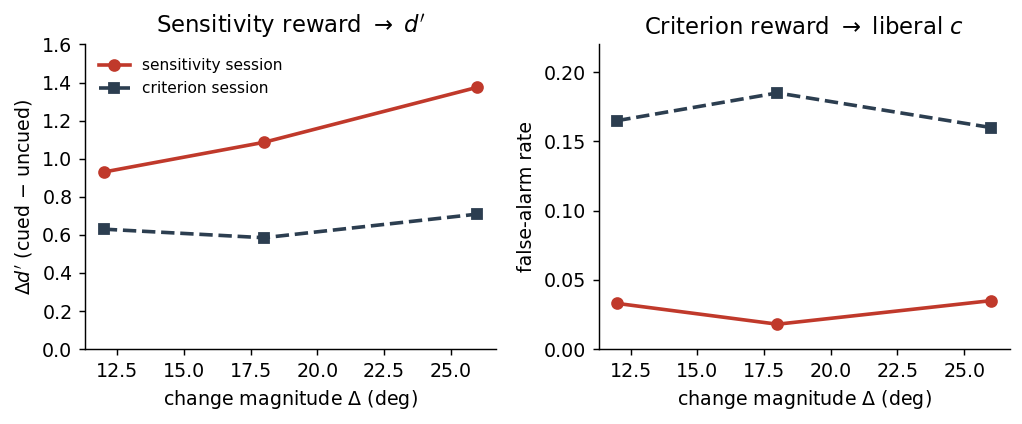
\includegraphics[width=0.86\linewidth]{figs/luo_repro}
  \caption{\textbf{(Preliminary; cued variant.)} \textbf{The reward-structure manipulation
    reproduces the Luo--Maunsell sensitivity/criterion double dissociation.} Across all three
    change magnitudes, the \emph{sensitivity} session (value concentrated at one
    location) yields a larger sensitivity gap ($\Delta\dprime$, left) at a
    \emph{low} false-alarm rate (right), whereas the \emph{criterion} session (global
    hit/correct-rejection reward) yields a smaller sensitivity gap but a \emph{high}
    false-alarm rate. At the near-threshold magnitude $\Delta = 18^\circ$:
    $\Delta\dprime = 1.09$ at $\mathrm{FA} = 0.02$ (sensitivity) versus
    $\Delta\dprime = 0.59$ at $\mathrm{FA} = 0.18$ (criterion).}
  \label{fig:luo_repro}
\end{figure}

That the two conditions differ in $\dprime$ and criterion-related false alarms is the
model's preliminary analogue of the central Luo and Maunsell result: the task directly
operationalizes a perceptual-stage sensitivity endpoint and a decision-stage criterion
endpoint, and the reward regime is the manipulated task factor. Both checkpoints were
trained with the same temporal JEPA auxiliary objective (loss weight $0.5$) as well as reinforcement; the
comparison does not attribute their learned representations to reward alone
\cite{luo_maunsell2018_criterion_sensitivity}. It also completes the within-task
picture of Section~\ref{sec:detection}: there, a graded attention clamp moved
criterion in the model and, through the attention-mediated read-out, sensitivity as
well; here, the animal's own reward manipulation elicits the \emph{selective} versions
of those two movements without any external clamp, showing that the model
reorganizes its attention endogenously to match the payoff.

\subsection*{Localizing the two effects: decision-stage criterion, attentional-gain
             sensitivity}

Reproducing the behavioral dissociation invites the mechanistic question the
electrophysiology asked: \emph{where} does each effect live? We localize each
component by measuring the model's own attention --- the fraction of priority placed
on the rewarded location --- in each session, and asking which manipulation changes
attention and which does not.

\paragraph{The criterion effect is decision-stage.} The criterion session raises the
false-alarm rate through a shift in the model's \emph{decision}, not its attention.
The read-out's declare bias at the change frame --- the actor's preference for
declaring a change over continuing to wait --- moves sharply toward reporting, from
$-15.4$ in the sensitivity session to $-3.6$ in the criterion session; it is this
liberal shift that inflates the false-alarm rate. Crucially, the shift is \emph{not}
accompanied by a withdrawal of attention: the model's attention to the cued location is
if anything marginally \emph{higher} in the criterion session ($\alphacued = 0.55$)
than in the sensitivity session ($0.46$; uniform $= 0.25$). The global reward therefore
does not change where the model looks; it changes only how readily the model converts
the evidence it has into a ``change'' declaration. This pattern localizes the measured criterion contrast to the decision read-out rather
than to a lower cued allocation in the priority map --- a model-level counterpart of the finding that
the criterion component is \emph{absent} from visual cortex and appears instead in
decision-related structures such as lateral prefrontal cortex
\cite{luo_maunsell2018_criterion_sensitivity}, and consistent with the criterion
movement being present in the model regardless of how attention is allocated
(Section~\ref{sec:detection}).

\paragraph{The sensitivity localization is carried by cue-anchored attention.} The
model does deploy spatial attention to the monitored location --- it places
substantial priority on the cued cell, $\alphacued = 0.46$--$0.55$ against a uniform
baseline of $0.25$ --- and this attention to the cued location is what yields the
higher cued-than-uncued sensitivity that defines the sensitivity component. Here,
however, we report the limitation plainly rather than overstate the match to cortex.
In the monkey, the sensitivity manipulation steers attention \emph{specifically to the
rewarded location}: gain is retargeted to where value is concentrated. In the model,
attention is instead \emph{cue-anchored}: it attends the cued location in both
sessions and does \emph{not} additionally concentrate attention on the
reward-relevant location in the sensitivity session beyond what the spatial cue
already commands (if anything the cued allocation is marginally larger in the criterion
session). The sensitivity dissociation therefore emerges behaviorally, and it rides on
genuine spatial attention to the cued location
\cite{mcadams_maunsell1999_v4_tuning,reynolds_heeger2009_normalization,%
sani2017_temporal_v4_gain}, but that attention is bound to the spatial cue rather than
being flexibly steered by the reward map --- the signature of the model's reflexive,
cue-driven read-out (cf.\ the transient-then-released attention time-course and the
value-blindness of the priority map, Section~\ref{sec:detection}).

\begin{figure}[t]
  \centering
  % FIGURE fig:luo_mechanism — attention on cued location + declare bias per session,
  % from luo_mechanism.py (affine_ew, no-change trials). alpha_c 0.46 sens / 0.55 crit;
  % declare bias -15.4 sens / -3.6 crit.
  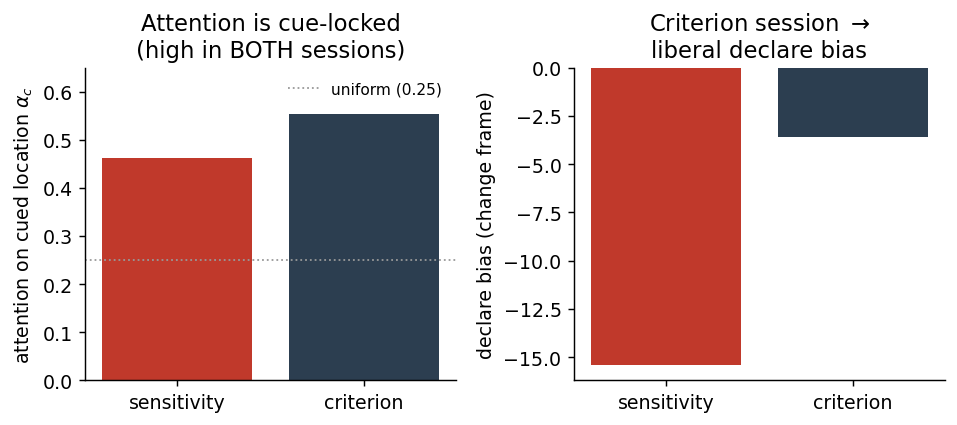
\includegraphics[width=0.82\linewidth]{figs/luo_mechanism}
  \caption{\textbf{(Preliminary; cued variant.) Localizing the two components (mechanism).} Left: attention to the
    cued location is high in \emph{both} sessions ($\alphacued = 0.46$ sensitivity,
    $0.55$ criterion; uniform $= 0.25$) --- the model's spatial attention is
    cue-anchored, not steered by the reward map. Right: the criterion session shifts
    the read-out's declare bias toward reporting (from $-15.4$ to $-3.6$), the
    decision-stage change that produces the high false-alarm rate. The criterion effect
    is thus a decision-stage bias shift with attention if anything slightly higher, not
    lower; the sensitivity dissociation rides on cue-anchored attention.}
  \label{fig:luo_mechanism}
\end{figure}

\subsection*{Interpretation}

Two conclusions follow, one positive and one qualifying. Positively, the preliminary
cued analogue directly measures a sensitivity endpoint ($\dprime$ at low false-alarm
cost) and a criterion endpoint (false-alarm rate with a smaller sensitivity change)
under two reward regimes. The accompanying read-outs associate the criterion contrast
with a declare-bias shift and show cue-anchored spatial attention in both checkpoints.
This two-endpoint distinction parallels the one that motivated the primate work and that
distinguishes the visual-cortical (sensitivity) from the decision-related (criterion)
locus of attentional modulation \cite{luo_maunsell2018_criterion_sensitivity,CohenMaunsell2009}. The qualification is
that the model's sensitivity gain is cue-locked: it arises through gain, as in the
animal, but the gain follows the spatial cue rather than being freely retargeted to a
reward-defined location. The model thus reproduces a behavioral contrast while realizing only a cue-anchored
version of the flexible, value-steered gain that the monkey
deploys. Both the success and its boundary are informative: they identify the reward
manipulation as sufficient to separate the two measured SDT endpoints across these
jointly RL--JEPA-trained checkpoints (auxiliary weight $0.5$), and they pinpoint reward-flexible spatial steering of gain --- as
opposed to cue-locked orienting --- as the specific capacity that the model's
read-out lacks. Whether a read-out whose gain channel could be steered by the
maintained value signal, rather than anchored to the spatial cue, would confine
sensitivity gain to the reward-relevant location, closing this gap, is
a direct prediction for future work; the timing dependence of such gain
\cite{ghose_maunsell2002_task_timing} and its feature specificity
\cite{treue_martinez_trujillo1999_feature_attention} are the natural next tests.
